\chapter{Especificação de Requisitos}
\label{sec:requisitos}

O processo de especificação de requisitos é crucial para o desenvolvimento de um projeto de \textit{software}, devendo dar atenção tanto aos requisitos funcionais como aos requisitos não funcionais.

Este capítulo apresenta os requisitos que foram identificados e analisados para a plataforma e define um conjunto de diretrizes que devem ser seguidas durante o desenvolvimento do projeto. Estes requisitos foram definidos e identificados com base em reuniões com o os responsáveis pelo projeto, nas necessidades que vão ao encontro do produto e na análise de soluções, atualmente no mercado, que partilham funcionalidades semelhantes com a plataforma que vai ser desenvolvida

Este capítulo divide-se em 3 secções. A secção \ref{requisitos:tiposutilizadores} identifica as principais partes envolventes no projeto. A secção \ref{rnf} e \ref{rf} descrevem,  detalhadamente, os requisitos não funcionais e funcionais, respectivamente. Por fim temos a secção \ref{prototipagem} que apresenta uma prototipagem de baixo nível, que com auxílio de breves descrições representa o fluxo da plataforma.


\section{Tipos de Utilizadores}
\label{requisitos:tiposutilizadores}

O objetivo desta secção é identificar, não necessariamente um problema, mas sim, através de uma estratégia de inbound marketing, uma forma de melhorar a experiência dos utilizadores proporcionando-lhes conteúdo que eles valorizam. Para melhor entender as necessidades do software é necessário fazer um estudo e tentar identificar os tipos de utilizadores finais, os seus comportamentos e fluxos de trabalho.


\subsection{\textit{Stakeholders}}

As principais partes envolventes neste projeto são, o proprietário do produto, os utilizadores principais e os utilizadores secundários. Como resultado, os tipos de utilizadores serão baseados num público considerado ideal, em especulações e dados reais.


\subsection{Proprietário do produto}

O proprietário do produto é o Sr. Pedro Girão, \acrshort{ceo} na 10.digital. O aluno irá fazer o levantamento dos requisitos para o projeto que serão validados pelo proprietário do produto.

\subsection{Utilizadores primários}

A plataforma 10.quest tem dois tipos de utilizadores primários. Os primeiros são os utilizadores que irão utilizar o \textit{backoffice} da plataforma que fornece uma série de funcionalidades para criar campanhas. Através destas campanhas, os dados recolhidos são tratados e estes utilizadores conseguem filtrar e segmentar as \textit{leads} através de perfis de personalidade. O segundo tipo de utilizadores primários são os utilizadores finais. Estes irão participar nas campanhas (i. e. formações, questionários de personalidade e/ou concursos) criadas pelo utilizador do \textit{backoffice}.


\subsection{Utilizadores secundários}

Considerando o impacto que pode ter no seu fluxo de trabalho e produtividade geral no seu departamento, e apesar de não serem utilizadores diretos, todo o suporte e manutenção fornecida pela 10.digital, faz com que as pessoas responsáveis sejam \textit{stakeholders}.
Outras entidades envolventes serão as responsáveis pela criação dos conteúdos que serão utilizados na plataforma.


\section{Requisitos Não Funcionais}
\label{rnf}

Os requisitos não funcionais dizem respeito aos atributos de qualidade da plataforma e foram identificados durante a fase de planeamento, adequando-se às necessidades do cliente e à natureza do produto. A lista de requisitos não funcionais é a seguinte:

\begin{itemize}
	\item \textbf{RNF01 - Segurança}
	\subitem - Um utilizador tem de estar autenticado para conseguir utilizar as funcionalidades da plataforma e apenas tem acesso a dados associados à sua conta. A comunicação com o \acrshort{tcg} será controlada com \textit{tokens}, para se controlar o acesso aos dados (i. e. um utilizador, autenticado ou não, não consegue efectuar pedidos de dados de outros utilizadores).
	\subitem - Medição: Testes de segurança.
	
	\item \textbf{RNF02 - Usabilidade} 
	\subitem - Um utilizador novo deve conseguir utilizar a plataforma (i. e. dominar todas as funcionalidades principais) em menos de 1 hora.
	\subitem - Medição: Testes de usabilidade
	
	\item \textbf{RNF03 - Disponibilidade}
	\subitem - Sem contar com falhas de rede, o sistema deve garantir uma disponibilidade  igual ou superior a 98\%.
	\subitem - Medição: Arquitetura de Software.
	
	\item \textbf{RNF04 - Desempenho}
	\subitem - A plataforma não deve demorar mais do que 4 segundos a executar um pedido efetuado pelo utilizador sendo que nos primeiros 2 segundos já deve mostrar alguma informação.
	\subitem - Medição: Testes de stress.
	
	\item \textbf{RNF05 - Robustez}
	\subitem - O sistema deve ser tolerante a falhas, erros e outras condições anormais. Eventos como falhas em pedidos à base de dados ou ao \acrshort{tcg}, \textit{inputs} inválidos, falhas de rede, dados inválidos etc., devem ser tratados de forma a não ter impacto negativo na plataforma.
	\subitem - Medição: Testes de \textit{White Box} e \textit{Black Box}.
\end{itemize}


\section{Requisitos Funcionais}
\label{rf}

Nesta secção serão analisados e detalhados todos os requisitos funcionais da plataforma.

Numa primeira fase serão descritos os vários diagramas que representam todos os requisitos funcionais do sistema, seguindo a legenda da Figura \ref{fig:rf-legenda}. Estes diagramas têm como principal objetivo contextualizar e dar uma visão global de todos os requisitos do sistema. É ainda de notar que para diminuir a complexidade e facilitar a compreensão dos diagramas, os requisitos de menor dimensão que não justificam a criação de um caso de uso estão nos diagramas para complementar alguns casos de uso (i. e. requisitos de maior relevância) contudo estão identificados com uma cor diferente. Desta forma é possível focarmo-nos apenas nos requisitos de maior relevância.

\begin{figure}[ht!]
	\begin{center}
		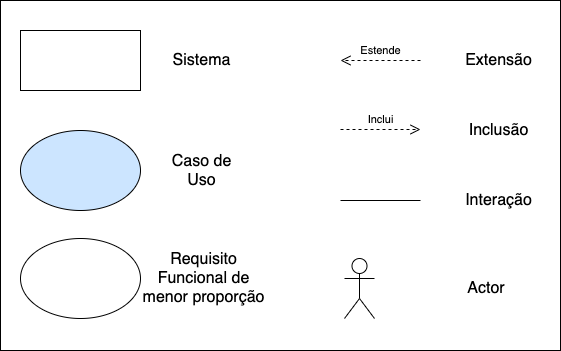
\includegraphics[width=0.7\textwidth]{img/rf/legenda}
		\caption{Legenda dos diagramas}
		\label{fig:rf-legenda}
	\end{center}
\end{figure}

Numa segunda fase serão analisados os graus de prioridade de cada requisito, consoante a sua importância para o projeto e por fim será feita uma descrição detalhada (i. e. especificação do requisito) de cada requisito através de casos de uso. É de notar que parte do grande trabalho da análise do grau de prioridade dos requisitos será imediato devido às decisões por parte do cliente.

Desta forma será claro para o leitor, mas em especial para a equipa de desenvolvimento, o comportamento que o sistema terá de cumprir. Os casos de uso serão detalhados consoante a seguinte estrutura:

\begin{itemize}
	\item \textbf{ID:} ID do caso de uso.
	\item \textbf{Ator:} Responsável pela realização do caso de uso.
	\item \textbf{Prioridade:} Representa a prioridade do caso de uso baseada nas decisões do cliente, visão dos stakeholders e no funcionamento do sistema. As prioridades foram classificadas por:
	\begin{itemize}
		\item \textbf{\textit{Must Have}:} Como o próprio nome indica, os requisitos \textit{Must} são os requisitos com maior prioridade. \textit{"As a rule, product inception depends entirely on defining must-haves using such pointers as ‘required for launch’, ‘required for safety’, ‘required for validation’, ‘required to deliver a viable solution’, etc."}\cite{railsware}. Todos os requisitos categorizados como \textit{Must Have}, são de implementação obrigatória pela equipa de desenvolvimento, uma vez que, sem eles o projeto fica paralisado.\textit{ "Can we move forward with the project if this task is undone? – if \textbf{NO}, it’s \textbf{MUST}"}\cite{railsware}.
		\item \textbf{\textit{Should Have}:} Os requisitos \textit{Should} são requisitos que também têm uma elevada prioridade, ou por outras palavras, estão apenas um passo abaixo dos requisitos \textit{Must}.
		Não são requisitos considerados vitais contudo adicionam valor significativo.\textit{ "Will we move forward with the project if this task is done a bit later? – if \textbf{YES}, it’s \textbf{SHOULD}"}\cite{railsware}.
		\item \textbf{\textit{Could Have}:} Os requisitos \textit{Could} são requisitos com menos importância e impacto que os anteriores. Pode-se dizer, por outras palavras, que são requisitos \textit{Nice to have} e tipicamente só são implementados se houver tempo para tal. \textit{ "Can we sacrifice this task till deadline? – if \textbf{YES}, it’s \textbf{COULD}"}\cite{railsware}.
		\item \textbf{\textit{Won't Have}:} Os requisitos \textit{Won't} são os requisitos com menor prioridade. Os requisitos categorizados com esta prioridade, tipicamente não são implementados no tempo estipulado para o projeto. Alguns requisitos são priorizados no futuro, outros nunca chegam a ser implementados. \textit{ "Can we go back to it when things go better? – if \textbf{YES}, it’s \textbf{WON’T}"}\cite{railsware}.
	\end{itemize}
	\item \textbf{Descrição:} Uma breve contextualização do caso de uso.
	\item \textbf{Pré-condições:} Conjunto de condições necessárias para realizar o caso de uso.
	\item \textbf{Estímulo:} Casos de uso responsáveis pela ativação do caso de uso.
	\item \textbf{Fluxo Principal:} Descrição detalhada de todos os passos para a realização do casos de uso.
	\item \textbf{Fluxo de Exceção:} Descrição detalhada do comportamento do sistema quando o caso de uso não for realizado com sucesso.
	\item \textbf{Observações:} Observações adicionais e relevantes para o desfecho do caso de uso.
\end{itemize}

\newpage

\subsection{Diagrama de contexto}
\label{d:contexto}
\begin{figure}[ht!]
	\begin{center}
		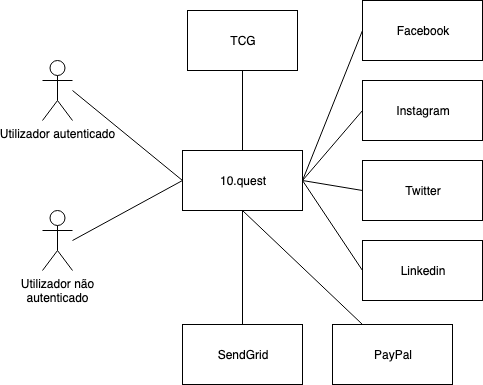
\includegraphics[width=0.6\textwidth]{img/rf/10quest}
		\caption{Diagrama de contexto}
		\label{fig:rf-10quest}
	\end{center}
\end{figure}

A 10.quest, tal como referido nos capítulos anteriores, é uma plataforma de inbound marketing que permite aos utilizadores criar campanhas e tratar a informação recolhida nas mesmas. 
Estas campanhas poderão ser partilhadas nas redes sociais (i. e. utilizando a API do Facebook, Instagram e Twitter) através de \textit{landing pages}. Estas \textit{landing pages} terão um pequeno formulário que necessita das informações básicas do utilizador final para que, automaticamente, as formações, questionários de personalidade e/ou concursos (i. e. campanhas) sejam enviados por mail para os inscritos, utilizando o sistema externo SendGrid.

Tal como referido no Capítulo \ref{sec:estado-arte}, o \acrshort{tcg} é um produto desenvolvido pela 10.digital e encontra-se atualmente no mercado. Algumas das funcionalidades fundamentais da plataforma a desenvolver já estão implementadas no \acrshort{tcg}  e por isso mesmo haverá uma integração com o mesmo para aproveitar todas estas funcionalidades necessárias.


\newpage

\subsection{Diagrama de Alto Nível}
\label{d:altonivel}
\begin{figure}[ht!]
	\begin{center}
		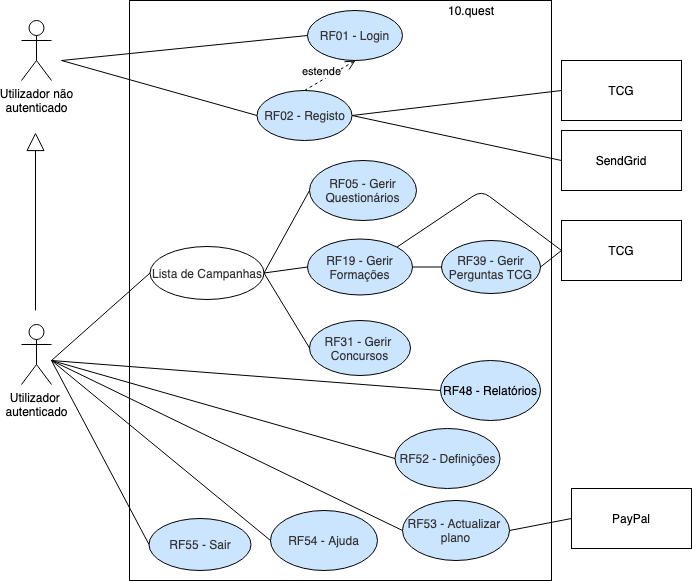
\includegraphics[width=0.8\textwidth]{img/rf/alto-nivel}
		\caption{Diagrama de Alto Nível}
		\label{fig:rf-alto-nivel}
	\end{center}
\end{figure}

Um utilizador para aceder a todas as funcionalidades da plataforma terá de primeiro realizar a autenticação (\textbf{RF01 - Login}). Caso ainda não tenha uma conta registada terá de o fazer. Assim que a conta for criada é enviada uma notificação para o email do utilizador, recorrendo ao sistema externo SendGrid. Por questões de segurança e confidencialidade dos dados, no acto do registo, a informação do utilizador será enviada e guardada na base de dados do \acrshort{tcg}, para que mais tarde todos os pedidos REST possam ser validados.

Depois de um utilizador se autenticar, será direcionado para a página inicial. A partir daqui o utilizador tem acesso à sua lista de campanhas (i. e. questionários, formações e concursos) podendo gerir as mesmas, bem como aceder às definições, atualizar o plano da conta, utilizar o suporte da plataforma e terminar sessão.
Ainda na página inicial da plataforma, onde se encontram listados todos os tipos de campanhas do utilizador da plataforma, será exibido o estado de cada campanha e data de término, se for o caso, para ajudar o utilizador a perceber de forma rápida o estado das mesmas.

\newpage

\subsection{Diagrama Registo}
\label{d:registo}
\begin{figure}[ht!]
	\begin{center}
		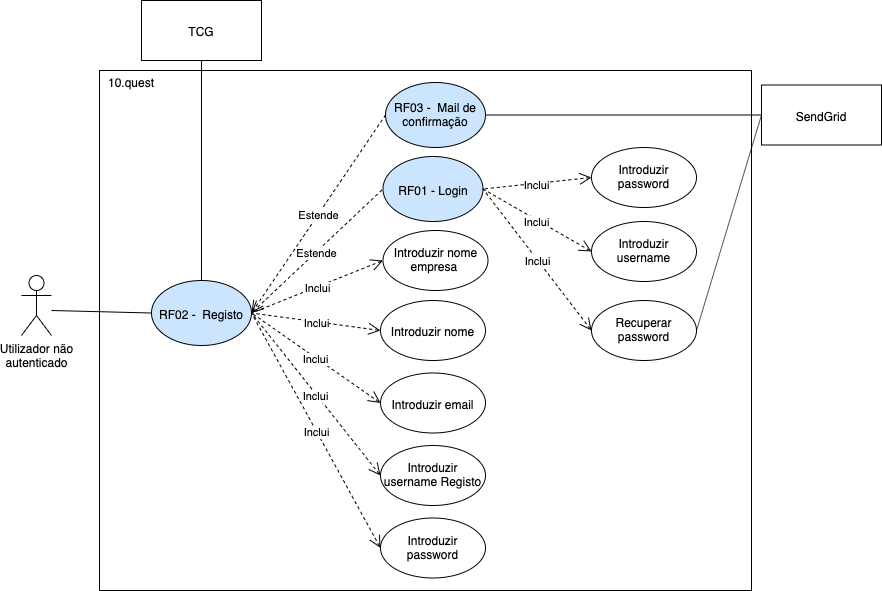
\includegraphics[width=1\textwidth]{img/rf/registo}
		\caption{Diagrama Registo}
		\label{fig:rf-registo}
	\end{center}
\end{figure}

Para se efetuar um registo é necessário introduzir o nome da empresa, nome do utilizador, email, \textit{username} e \textit{password}. De seguida é enviado um mail de validação para o email associado à conta.

Depois de validada a conta do utilizador, este consegue efetuar o \textit{login} na plataforma.



\newpage

\subsection{Diagrama Gerir Perguntas de Formação}
\label{d:perguntastcg}
\begin{figure}[ht!]
	\begin{center}
		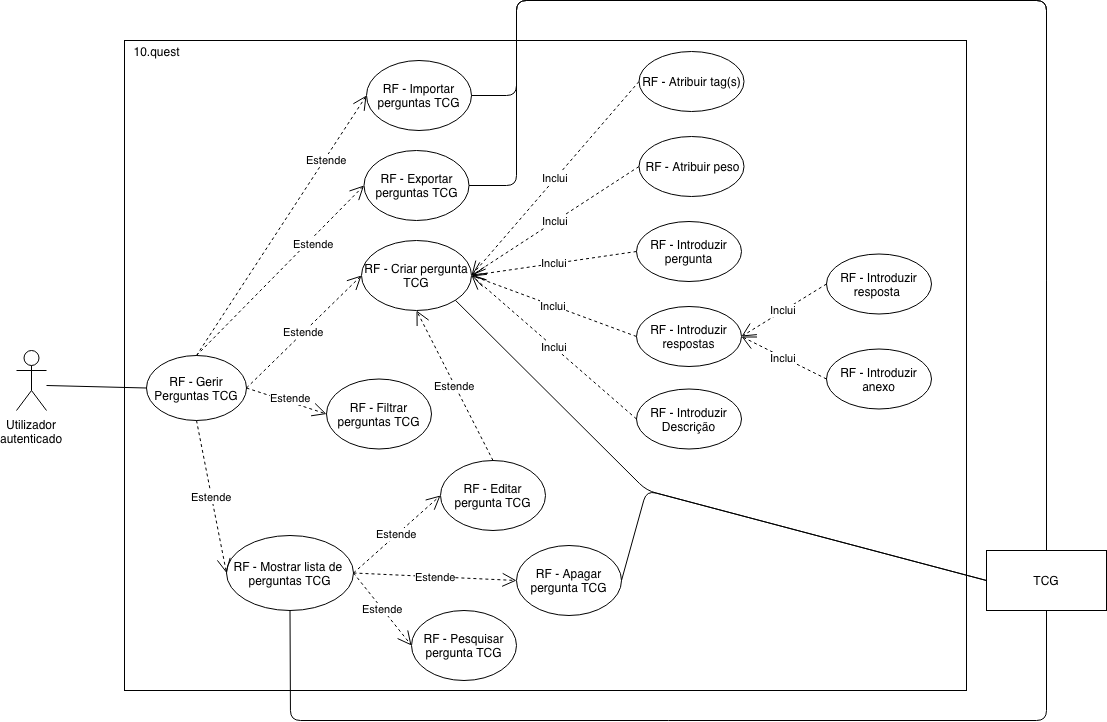
\includegraphics[width=1\textwidth]{img/rf/gerir-perguntas-tcg}
		\caption{Diagrama Gerir Perguntas de Formação}
		\label{fig:rf-gerir-perguntas-tcg}
	\end{center}
\end{figure}

No \acrshort{tcg}, tal como referido no anexo \ref{sec:TCG}, a criação de questões é isolada da criação de formações. Esta abordagem acarreta uma série de vantagens, referidas no Capítulo \ref{sec:TCG}, e neste sentido, este será o modelo seguido. Dito isto, é necessário primeiro criar questões para que se possa ter conteúdos para as formações. 

É ainda de notar que por uma questão de terminologia, na plataforma a desenvolver, as Perguntas de Formação são equivalentes às questões no \acrshort{tcg}, pelo simples facto de não se confundir com elementos relacionados com os questionários de personalidade.

Na gestão de perguntas de formação, um utilizador consegue listar todas as perguntas (\textbf{RF45 - Mostrar lista de perguntas de formação}) associadas à sua conta (i. e. criadas por ele) e pode também criar uma nova pergunta (\textbf{RF42 - Criar pergunta de formação}). Para editar uma pergunta (\textbf{RF46 - Editar pergunta de formação}) é necessário aceder à mesma através da lista, sendo que é possível organizar e pesquisar por nome ou tag, e é ainda possível selecionar múltiplas perguntas de formação para eliminar (\textbf{RF47 - Apagar pergunta de formação}). As perguntas podem também ser importadas e exportadas através de uma \textit{spreadsheet}.

Para um criar uma pergunta (\textbf{RF42}), o utilizador precisa de atribuir uma tag, nova ou existente, introduzir a pergunta e as respostas. Cada pergunta tem que ter obrigatoriamente uma resposta certa e pelo menos uma resposta errada, sendo estas compostas pela resposta e um anexo opcional que pode ser uma imagem ou vídeo.



\newpage

\subsection{Diagrama Gerir Formações}
\label{d:formacoes}
\begin{figure}[ht!]
	\begin{center}
		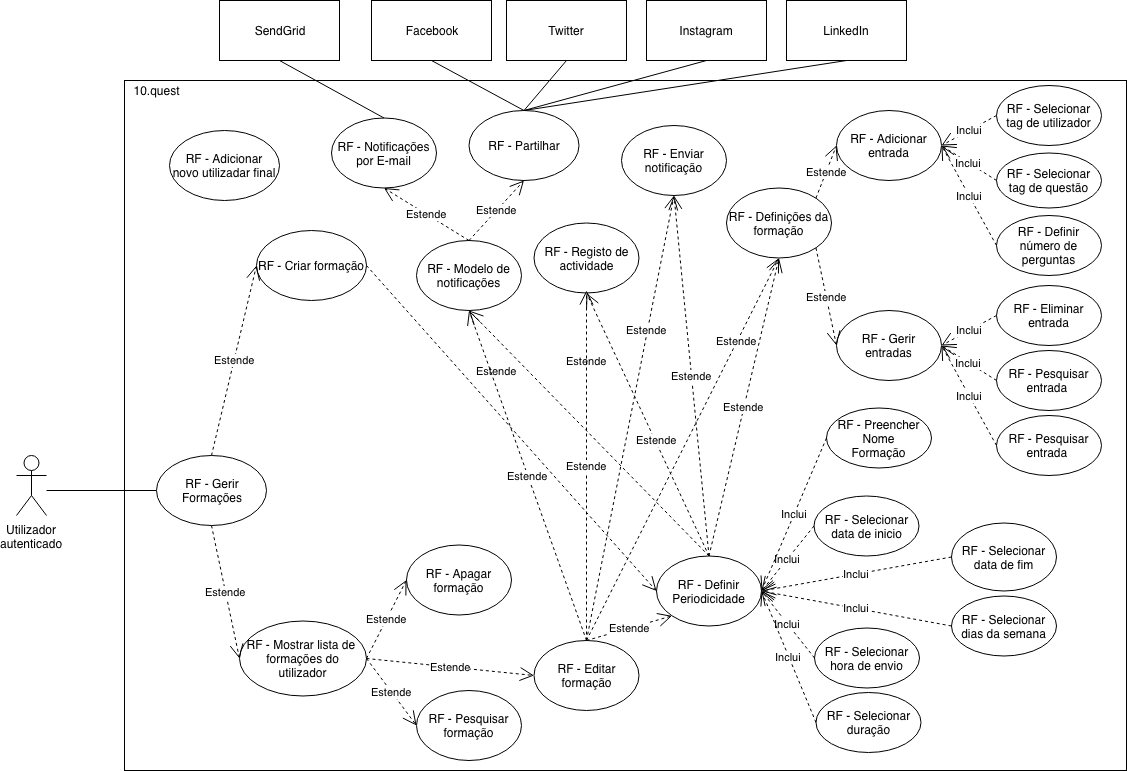
\includegraphics[width=1\textwidth]{img/rf/gerir-formacoes}
		\caption{Diagrama Gerir Formações}
		\label{fig:rf-gerir-formacoes}
	\end{center}
\end{figure}

Quase todas as funcionalidades necessárias para a gestão de formações já estão implementadas no \acrshort{tcg}. Neste sentido terá que ser apenas garantido um conjunto de requisitos que permita ao utilizador reunir as condições necessárias para utilizar as capacidades do TCG através de pedidos REST. Isto implica ter uma interface completa no lado do 10.quest e selecionar quais os dados a guardar no 10.quest e no \acrshort{tcg}, respetivamente, garantindo sempre a sincronização dos dados.

Na gestão de formações um utilizador consegue listar todas as formações associadas à sua conta (\textbf{RF27 - Mostrar lista de formações do utilizador}) e pode também criar uma nova formação (\textbf{RF20 - Criar formação}).
Para criar uma formação (\textbf{RF20}) o utilizador terá, numa primeira instância, de atribuir um nome e definir a periodicidade (i. e. preencher a hora de envio, dias da semana,  duração e validade) (\textbf{RF21 - Definir periodicidade}). 
Numa segunda fase, o utilizador, através do requisito \textbf{RF - Definições da formação} consegue adicionar e gerir entradas de perguntas de formações (\textbf{RF25 - Adicionar entrada de perguntas} e \textbf{RF26 - Gerir entradas de perguntas}, respetivamente). É através destas entradas que o utilizador da plataforma associa perguntas à formação. Para adicionar uma entrada (\textbf{RF25 - Adicionar entrada de perguntas} ) o utilizador da plataforma seleciona as perguntas que deseja através de tags (i.e. as perguntas com as tags respectivas são associadas) e o número de perguntas que o utiliador final irá receber, com esse mesmo perfil de tags.

Por fim o utilizador pode partilhar a formação (\textbf{RF56 - Partilhar}). As inscrições numa formação serão feitas através de uma \textit{landing page} que pode ser personalizada no requisito \textbf{RF08 - Landing Page} e enviadas para o email introduzido no mini formulário da \textit{landing page}. Este mail com o link para a formação, pode ser personalizado no requisito \textbf{RF09 - Notificações por E-mail}. 

É de notar que, através do requisito \textbf{RF29 - Adicionar novo utilizador final TCG}, sempre que um utilizador final se inscreve numa formação através da \textit{landing page}, o sistema, de forma automática, envia os dados para o \acrshort{tcg} para que este utilizador possa começar a receber a formação por email. Outro requisito da responsabilidade do sistema é o \textbf{RF30 - Notificar utilizadores finais TCG}, que respeitando a periodicidade definida na criação da formação, envia a formação para todos os inscritos.



\subsection{Diagrama Gerir Questionários de Personalidade}
\label{d:quests}
\begin{figure}[ht!]
	\begin{center}
		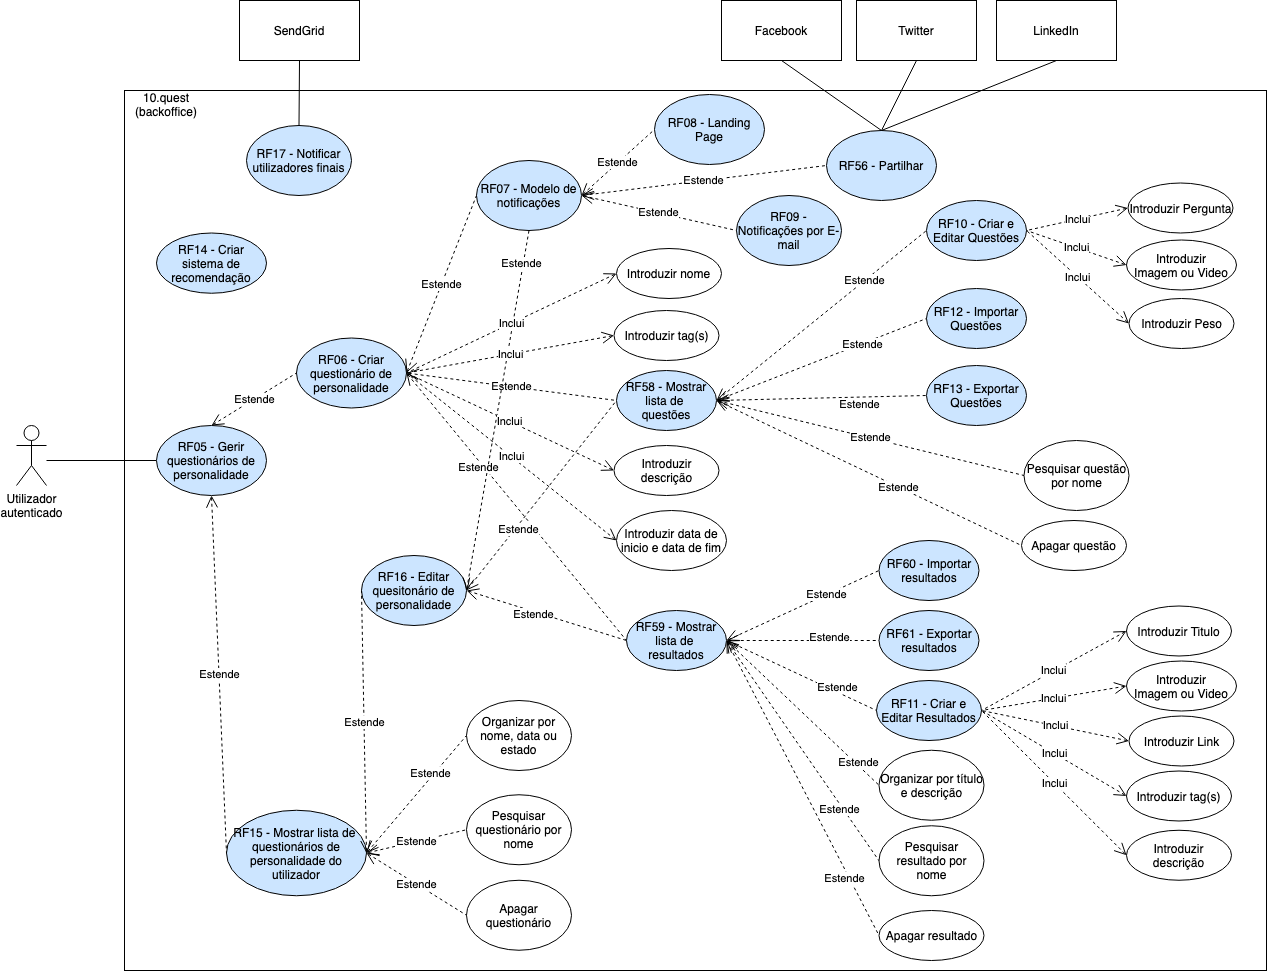
\includegraphics[width=1\textwidth]{img/rf/gerir-quest}
		\caption{Diagrama Gerir Questionários}
		\label{fig:rf-gerir-quest}
	\end{center}
\end{figure}

Na gestão de questionários de personalidade, à semelhança da gestão de formações, é feita uma listagem dos questionários (\textbf{RF15 - Mostrar lista de questionários de personalidade do utilizador}) e o utilizador tem a capacidade de criar (\textbf{RF06 - Criar questionário de personalidade}), eliminar, editar (\textbf{RF16 - Editar questionário de personalidade}) e pesquisar questionários pelo nome.
Na criação de um novo questionário de personalidade (\textbf{RF06}), numa primeira fase o utilizador tem de introduzir o nome do questionário, descrição, data inicio e data de fim e tags. Numa segunda fase o utilizador, terá de criar um conjunto de questões (\textbf{RF10 - Criar questões}) e gerar um série de resultados (\textbf{RF11 - Criar resultados}). Para manter a criação do questionário o mais intuitivo e amigo do utilizador, não há uma ordem especifica para a criação de questões e resultados sendo que a qualquer momento o utilizador da plataforma pode voltar a adicionar, editar ou eliminar uma questão ou resultado. 

Quando o utilizador abre um questionário de personalidade, para além das informações básicas da campanha, tem a lista de questões (\textbf{RF56 - Mostrar lista de questões}) e a lista de resultados (\textbf{RF57 - Mostrar lista de resultados}). Em ambas as listas é possível organizar e pesquisar pelo nome, apagar um elemento, importar e exportar questões e resultados respectivamente, através de uma \textit{spreadsheet} (\textbf{RF12 - Importar questões} e \textbf{RF13 - Exportar questões}; \textbf{RF59 - Importar resultados} e \textbf{RF58 - Exportar resultados}).

Para criar uma questão (\textbf{RF10 - Criar questões}), o utilizador terá de introduzir a pergunta, uma imagem ou video se desejar e um peso. O peso está associado ao impacto que a pergunta tem no calculo do resultado, que será explicado de seguida. 
Cada resultado terá de ter obrigatoriamente uma ou mais \textit{tags} associadas e um título, e opcionalmente uma descrição, um link e uma imagem ou video(\textbf{RF11 - Criar resultados}). À semelhaça das questões, a qualquer momento o utilizador pode editar um resultado.

O sistema de recomendação, o unico factor com que o utilizador da plataforma terá de se preocupar será o peso que atribui a cada pergunta, isto é, o impacto que cada pergunta tem no calculo do resultado final. No final de cada submissão por parte dos utilizadores finais (i. e. \textit{leads}) o sistema vai avaliar todas as respostas efectuadas pelo utilizador final e o calculo final será baseado na correspondência de tags e na pontuação. A correspondência de tags indica quais os resultados mais indicados e a pontuação ajuda a decidir quais os mais relevantes.

Através do requisito \textbf{RF18 - Adicionar novo utilizador final}, sempre que um utilizador final se inscreve num questionário através da \textit{landing page}, o sistema, de forma automática, guarda essa informação e recorrendo ao requisito \textbf{RF17 - Notificar utilizadores finais}, envia o questionário para o utilizador final.

\pagebreak

\subsection{Diagrama Gerir Concursos}
\label{d:concursos}
\begin{figure}[ht!]
	\begin{center}
		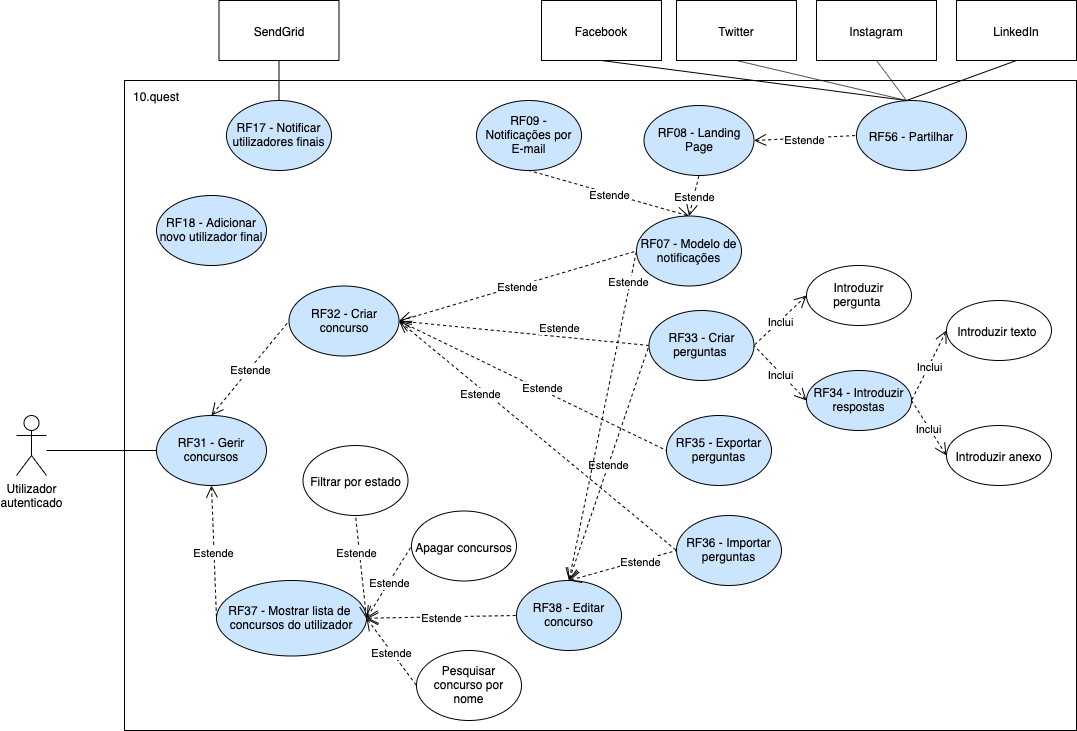
\includegraphics[width=1\textwidth]{img/rf/gerir-concurso}
		\caption{Diagrama Gerir Concursos}
		\label{fig:rf-gerir-concursos}
	\end{center}
\end{figure}


Na gestão de concursos, à semelhança da gestão de formações e questionários de personalidade, é feita uma listagem dos concursos (\textbf{RF37 - Mostrar lista de concursos do utilizador}) e o utilizador tem a capacidade de criar (\textbf{RF32 - Criar concurso}), eliminar, editar (\textbf{RF38 - Editar concurso}) e pesquisar questionários.

À semelhança das campanhas anteriores, na criação de concuros (\textbf{RF32 - Criar concurso}) , primeiro é necessário introduzir as definições básicas. O utilizador tem primeiro de introduzir o nome do concurso, uma descrição, uma data de inicio e uma data de fim e uma ou mais tags que irão ser associadas aos participantes (i.e. \textit{leads}).

Cada concurso tem uma lista de perguntas (\textbf{RF60 - Mostrar lista e perguntas}) criadas pelo utilizador(\textbf{RF33 - Criar perguntas}). Para cada pergunta o utilizador terá de introduzir pelo menos duas respostas (\textbf{RF34 - Introduzir respostas}), uma certa e uma errada, e opcionalmente pode anexar uma imagem ou video. As perguntas e respostas podem também ser importados e exportados através de uma  \textit{spreadsheet} (\textbf{RF36 - Importar perguntas} e \textbf{RF35 - Exportar perguntas}, respectivamente).

É importante referenciar que à semelhança da gestão de formações e questionários, é possível editar os conteúdos (i. e. perguntas, questões, \textit{landing pages}, email etc) contudo, assim que um concurso é publicado e passa a estar no estado \textit{online}, apenas as definições básicas da campanha, excepto as tags, podem ser editadas. 

Os concursos, tal como as restantes campanhas têm sempre um estado que pode variar entre:
\begin{itemize}
	\item Rascunho - O utilizador da plataforma não deu a campanha como concluída portanto o sistema assume que é rascunho.
	\item Concluido - O utilizador da plataforma marcou a campanha como concluída.
	\item \textit{Online} - Utilizador gerou a \textit{landing page} para partilhar a campanha.
	\item Fechado - A campanha chegou à data de fim.
\end{itemize}


\subsection{Diagrama Ajuda}
\label{d:ajuda}
\begin{figure}[ht!]
	\begin{center}
		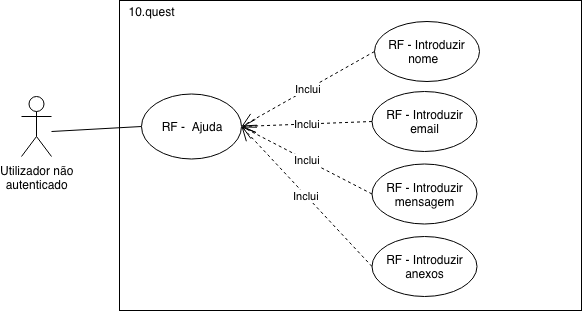
\includegraphics[width=1\textwidth]{img/rf/ajuda}
		\caption{Diagrama Ajuda}
		\label{fig:rf-ajuda}
	\end{center}
\end{figure}


O utilizador poderá, se assim o pretender, utilizar o suporte da plataforma. Em caso de dúvida ou esclarecimentos, enviar uma mensagem direta para a 10.digital. 

Para enviar uma mensagem é necessário introduzir o nome, email, mensagem e, caso o utilizador deseje, um ou mais anexos.

\newpage

\subsection{Diagrama Relatórios}
\label{d:relatorios}

\begin{figure}[ht!]
	\begin{center}
		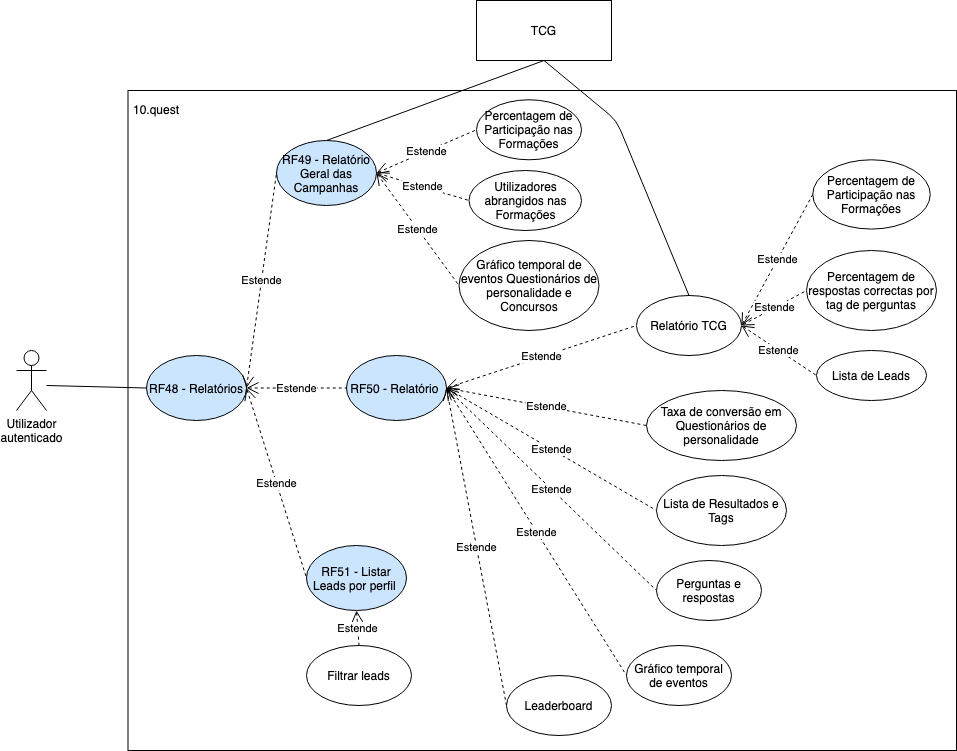
\includegraphics[width=1\textwidth]{img/rf/relatorio}
		\caption{Diagrama Relatórios}
		\label{fig:rf-relatorios}
	\end{center}
\end{figure}

Assim que uma campanha for publicada (i.e. o seu estado for online ou terminado), um utilizador pode gerar o relatório de dados. A secção de dados da plataforma mostra os resultados gerais sobre as campanhas (\textbf{RF49 - Relatório geral}) e permite também ao utilizador da plataforma gerar um relatório com informações mais detalhadas sobre uma campanha (\textbf{RF50 - Relatório}).

Como foi referido anteriormente, o utilizador da plataforma pode gerar um relatório (\textbf{RF50}) para uma campanha, online ou terminada, onde será exposto o resultadoso mesmo. As métricas analisadas relevantes para cada tipo de campanha são diferentes e por isso os relatórios serão diferentes nesse sentido.

Quando o utilizador da plataforma acede à secção dos relatórios (\textbf{RF48 - Relatórios}), será apresentado o relatório geral das campanhas (\textbf{RF49 - Relatório Geral das Campanhas}) e a lista de leads (\textbf{RF51 - Listar Leads}). O relatório geral das campanhas apresenta métricas relacionadas com tráfego de utilizadores finais (i.e. \textit{leads}) e na lista de leads, são apresentados todos os participantes qualificados, as suas informações básicas e o seu perfil traçado nas campanhas em que participou (i.e. todas as tags que tem associadas, permite traçar um perfil de personalidade). Na lista de leads é possível filtrar participantes qualificados por tags, ou por outras palavras, por um perfil de personalidade.
	
Para gerar um relatório mais detalhado o utilizador da plataforma terá de selecionar a campanha para o qual quer gerar o mesmo. No caso da campanha ser uma formação serão apresentados dados relaticos à participação dos utilizadores finais, percentagem de respostas correctas por tag e a lista de utilizadores finais (i.e. leads). Na lista de utilizadores finais, para cada lead diz: o nome, a média de questões por dia, percentagem de participação, total de respostas erradas, total de respostas correctas, respostas, percentagem de respostas correctas e o tempo total gasto a participar na formação. 
Nas restantes campanhas, isto é, questionários de personalidade e concursos, grande parte das métricas tiradas são comuns. Em ambas as campanhas é aprentado as perguntas e respostas de todas as leads, o funil de participação e o gráfico temporal de eventos. A lista de resultados e tags é somente apresentada para os questionários de personalidade e a tabela de classificações para os concursos. 

O Funil de participação é um modelo estratégico separado por camadas, que apresenta de forma visual a jornada do participante (i.e. lead) durante a campanha. Este fúnil segue a mesma ideia do fúnil e marketing\cite{f8}\cite{f9} em que. As camadas representadas no funil estão organizadas por ordem de eventos e são: Visitas na página de apresentação, registos na página de apresentação, participações e submissões.

O gráfico temporal de eventos é um gráfico que de forma temporal mostra o número de visualizações da página de apresentação, número de registos na campanha e o número de submissões.

É ainda de notas que todos os dados não relacionados com tráfego dão para ser exportados através de uma \textit{spreadsheet}.


\section{Mockups}
\label{prototipagem}

A criação de mockups/protótipos de baixa fidelidade, teve como principal objetivo representar a plataforma (i. e. todos os requisitos funcionais) de forma estática. Esta secção foi importante para conseguir visualizar a plataforma como um todo, facilitando a implementação, e também teve um papel importante na verificação dos requisitos levantados, satisfazendo todos os casos de uso descritos no Anexo \ref{a:cu}. Todos os mockups realizados encontram-se descritos no Anexo \ref{a:prototipos}.


%-------------------------------------------------------------------------------------------------
\blankpage
%-------------------------------------------------------------------------------------------------

\glsresetall